\chapter{Compilador}
\label{comp}

\lstset{commentstyle=\color{green},
keywordstyle=\color{blue},
stringstyle=\color{red},backgroundcolor=\color{white}}

O processo de compilação não é trivial, e é dividido em 3 estágios:
\begin{itemize}
    \item \textbf{análise léxica}: reconhece as ``palavras'' que compõe um programa,
    ignorando espaços em branco. É capaz de identificar números, 
    constantes, nomes de objetos e pontuação.
    Os termos são usados no estágio seguinte.

    \item \textbf{análise sintática}: reconhece a estrutura do programa, como
    as declarações dos objetos e as expressões matemáticas.
    A gramática \ref{grammar} é usada como base.

    \item \textbf{análise semântica e síntese}: gera todas as estruturas de dados
    necessárias para a visualização dos objetos.
    Verifica também a semântica do programa,
    detectando erros que não podem ser verificados com noções gramaticais.
\end{itemize}

A teoria de compiladores é essencial para esses estágios \cite{Dragon:1}.

\newpage

\section{Análise léxica}
A análise léxica tem a função de ler o código-fonte que descreve um programa
e abstrair as palavras e símbolos presentes.
Dessa forma, os estágios seguintes se beneficiam dessa abstração.
O analisador léxico é chamado de \textit{lexer}.

As palavras-chave, números, constantes, símbolos, etc. são chamados de lexemas.
Todo lexema deve pertencer a uma classe gramatical.
Por exemplo, o texto \texttt{"1024"} forma um lexema de 4 caracteres
e sua classe gramatical é \texttt{NUMBER}.
Conforme a classe, um lexema pode ter atributos.
No caso de \texttt{NUMBER}, o próprio número em forma de ponto flutuante é um atributo.
No caso de um símbolo como \texttt{";"}, não há atributos.

Um lexema, sua classe gramatical e seus atributos juntos formam um \textit{token}.

Os tipos de \textit{token} são:

\begin{table}[ht]
\caption{Tipos de \textit{token}}
\label{tokentypes}
\begin{centering}
\begin{tabularx}{\textwidth}{||c|X||}
\hline \texttt{COMMENT} & texto livre, começando com \texttt{"\#"} e
terminando com uma quebra de linha ou o fim do código-fonte.\\ 
\hline \texttt{FUNCTION} & identificador de função definida ou pré-definida.\\
\hline \texttt{NUMBER} & número de ponto flutuante.\\
\hline \texttt{VARIABLE} & identificador de variável de função.\\
\hline \texttt{CONSTANT} &identificador de constante definida ou pré-definida.\\
\hline \texttt{DECLARE} & identificador de tipo de objeto.\\
\hline \texttt{UNDEFINED} & identificador não definido ou a ser definido.\\
\hline \texttt{EOI} & fim do código-fonte, caractere nulo(0).\\
\hline Caso final & o lexema é um símbolo e seu tipo é o próprio símbolo.\\
\hline
\end{tabularx}
\end{centering}
\end{table}

A estrutura \texttt{Lexer}(\ref{lexer}) define o analisador léxico.
\lstset{language=c++}\code{files/lexer.txt}{Estrutura do \textit{lexer}}{lexer}

O \textit{lexer} lê os \textit{tokens} um de cada vez, da esquerda para a direita.
Essa estrutura guarda as seguintes informações sobre o \textit{token} atual:

\begin{table}[ht]
\caption{Estrutura do \textit{token}}
\label{token}
\begin{centering}
\begin{tabularx}{\textwidth}{||c|X||}
\hline \texttt{source} & \textit{string} do código-fonte inteiro. \\
\hline \texttt{lexeme} & aponta para o primeiro caractere do lexema atual(dentro da \textit{string} \texttt{source}) \\
\hline \texttt{length} & comprimento do \textit{token}. \\
\hline \texttt{lineno} e \texttt{column} & o número da linha e coluna do lexema. \\
\hline \texttt{type} & tipo do \textit{token}. \\
\hline \texttt{number} e \texttt{node} & atributos do \textit{token}.
No caso de um número, \texttt{number} é o atributo.
No caso de um identificador, \texttt{node} é sua posição na tabela de símbolos(\ref{table}),
contendo mais informações sobre o \textit{token}. \\
\hline \texttt{table} & tabela de símbolos compartilhada pelos estágios da compilação. \\
\hline
\end{tabularx}
\end{centering}
\end{table}

O \textit{lexer} tem apenas o método \texttt{advance}, que serve para avançar
para o próximo \textit{token}. O método também é usado para inicializar o
\textit{lexer} e obter o primeiro \textit{token} do código-fonte,
invocando-o com \texttt{lexeme=source} e \texttt{length=0}.

O método começa avançando a posição do \texttt{lexeme} a quantidade de
\texttt{length} caracteres à direita.
Em seguida, espaços em branco são ignorados: espaços, tabulações e quebras de linha.

Se o caractere em \texttt{lexeme} for \texttt{"\#"}, então o \textit{token} é um
comentário(tipo \texttt{COMMENT}),
que se estende até uma quebra de linha ou até o \texttt{EOI}, sem incluí-los.

Se o caractere for nulo(0), então o tipo do \textit{token} é \texttt{EOI} e \texttt{length=0}.
Isso faz com que o \textit{lexer} trave nesse \textit{token} e nunca mais avance.

Se o caractere for um dígito ou \texttt{"."}, então o \textit{token} é um número(tipo \texttt{NUMBER}),
e é lido pela função \texttt{sscanf} da linguagem C.

Se o caractere pertencer ao alfabeto dos identificadores,
então o \textit{lexer} o procura na tabela de símbolos obtendo o \texttt{node}.
Com esse nó, o tipo de \textit{token} e comprimento são obtidos.

Caso contrário, o \textit{token} é um símbolo, seu tipo é o próprio símbolo
e seu comprimento é 1.

\newpage

\section{Tabela de símbolos}
Os estágios da compilação compartilham uma tabela de símbolos,
que é inicializada com palavras-chave,
funções e constantes pré-definidas.
A tabela de símbolos define os atributos dos identificadores,
que são o tipo do \textit{token}, os argumentos da função e o índice do objeto.

A estrutura \texttt{Table}(\ref{table}) define a tabela de símbolos.
\lstset{language=c++}\code{files/table.txt}{Tabela de símbolos}{table}

Essa estrutura é uma árvore de prefixos(trie):
cada nó representa um identificador. Para encontrar um nó a partir
de um identificador, basta traçar um caminho a partir da raiz.
Os filhos de um nó correspondem a um caractere do alfabeto \texttt{a-zA-Z0-9}.
Os 26 primeiros filhos são \texttt{a-z}, os próximos 26 são \texttt{A-Z},
e os 10 últimos são \texttt{0-9}.
Assim, cada letra do alfabeto indica qual filho seguir.

O membro \texttt{character} representa a letra conforme o pai do nó.
Por exemplo, se o nó é o primeiro filho, então a letra é \texttt{a}.
Para a raiz, o caractere é nulo(0).
O membro \texttt{parent} é o pai do nó, ou nulo para a raiz.
Os nós \texttt{children[62]} são os $26+26+10$ filhos.
O tamanho do identificador é \texttt{length}, e seus atributos são
\texttt{type}, \texttt{argIndex} e \texttt{objIndex}.
O atributo \texttt{argIndex} representa os argumentos de uma função definida.
\texttt{type} sempre indica o tipo do \textit{token}.
\texttt{objType} representa o índice de um objeto.

O método \texttt{next} encontra o filho correspondente ao caractere \texttt{c},
e caso seja nulo, um novo filho é criado.
O método \texttt{procString} busca o identificador em \texttt{str} na árvore,
usando \texttt{next} para traçar o caminho correto.
O ponteiro \texttt{str} indica o início do identificador(dentro do código-fonte).
O método avança no máximo até o primeiro caractere fora do alfabeto
dos identificadores.
Se o indicador \texttt{match} estiver ativo, o método buscará o
maior identificador definido, se existir, ou o identificador todo, caso contrário.
Por exemplo(\texttt{match=true}) para \texttt{"sinx"},
o método encontra o identificador \texttt{"sin"}, que é uma função.
Ou seja, os identificadores não precisam estar separados por um espaço em branco,
caso não haja ambiguidade.
Se um objeto de nome \texttt{"sinx"} estivesse definido,
o método encontraria o identificador \texttt{"sinx"}, pois é maior.
Nesse caso, um espaço em branco faz diferença.

O método \texttt{initString} usa \texttt{procString}
para criar o identificador em \texttt{str},
inicializando seu tipo de \textit{token} com \texttt{type}.

Para o exemplo \ref{ex1}, a tabela é a trie ilustrada na Figura \ref{img:ex1table}.
\begin{figure}[!ht]
    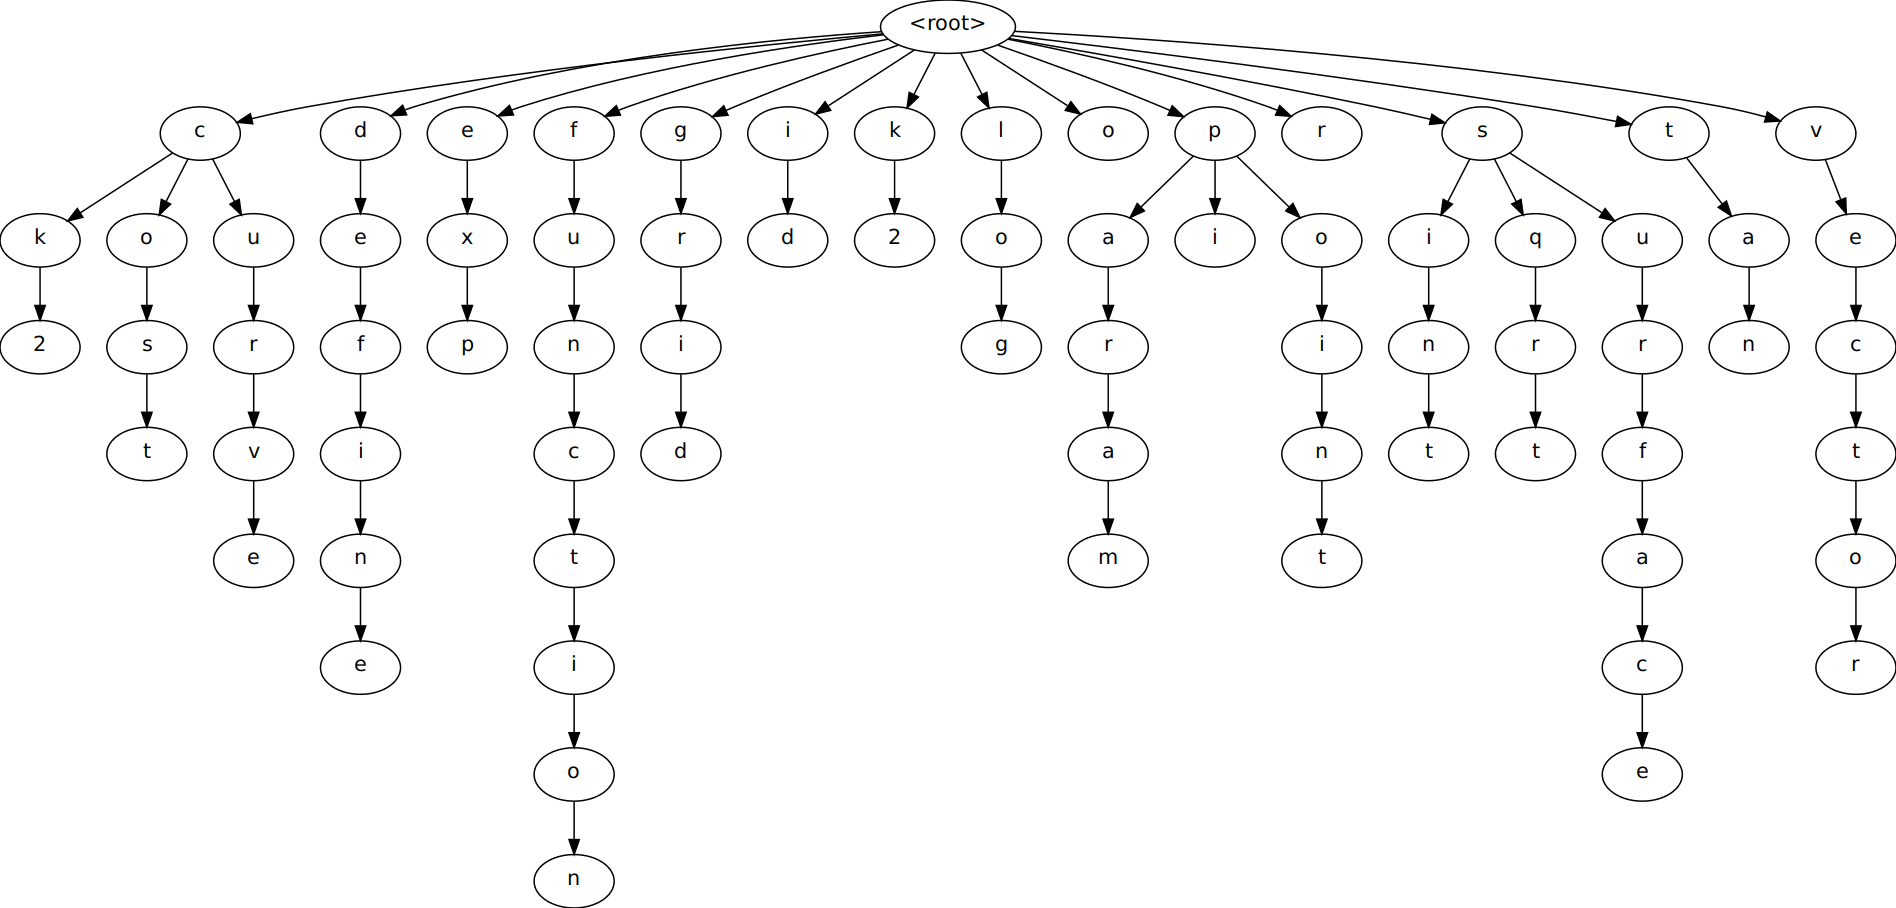
\includegraphics[width=\linewidth]{ex1table.png}
    \caption{Tabela de símbolos do Código \ref{ex1}}
    \label{img:ex1table}
\end{figure}

Nessa Figura, o nó correspondente ao termo \texttt{cos} indica \texttt{type=FUNCTION},
e para \texttt{k2}, \texttt{type=CONSTANT}.

\section{Análise sintática}
A análise sintática tem a função de identificar as estruturas sintáticas
presentes nos \textit{tokens} gerados pelo \textit{lexer}.
O gerador, no estágio seguinte, atribui um significado para as estruturas
sintáticas reconhecidas, gerando as estruturas de dados desejadas.
O analisador sintático é chamado de \textit{parser}.

\newpage
A gramática livre-de-contexto (\ref{grammar}) define as
regras gramaticais da linguagem.
\lstset{language=}\code{files/grammar.txt}{Gramática livre-de-contexto}{grammar}

A gramática consiste em diversas igualdades.
Os termos que aparecem no lado esquerdo de alguma igualdade
são chamados de não-terminais,
e representam um conjunto de sentenças(uma sentença é uma sequência de terminais).
Os outros termos, como \texttt{";"} e \texttt{id}, são terminais,
e correspondem a \textit{tokens}. Os termos \texttt{id}, \texttt{var},
\texttt{const}, \texttt{num}
e \texttt{func} representam qualquer \textit{token} do tipo indicado:
\texttt{UNDEFINED}, \texttt{VARIABLE}, \texttt{CONSTANT},
\texttt{NUMBER} e \texttt{FUNCTION} respectivamente.
Os termos \texttt{"param"}, \texttt{"grid"}, \texttt{"define"}, etc.
representam os \textit{tokens} do tipo \texttt{DECLARE}, que são os tipos de objeto.

Uma igualdade na gramática é dita uma produção para o não-terminal à esquerda.
O símbolo \texttt{"\textbar"}  abrevia uma produção alternativa. 
Por exemplo: \texttt{ADD = ADD + JUX | ADD - JUX | JUX}
é uma abreviação de \texttt{ADD = ADD + JUX},
\texttt{ADD = ADD - JUX} e \texttt{ADD = JUX}.
Uma produção pode ser a \textit{string} vazia, por exemplo: \texttt{PROG = DECL PROG | ;}
(o ponto e vírgula no final das igualdades pertence à meta-linguagem).

Uma produção significa que o não-terminal à esquerda pode ser substituído
pela forma sentencial à direita.
Uma forma sentencial é uma sequência de terminais e não-terminais.
Por exemplo, \texttt{ADD} pode ser substituído por \texttt{ADD + JUX}.
Nesse caso, \texttt{ADD} deriva \texttt{ADD + JUX}.
Para se obter um programa gramaticalmente válido,
o não-terminal inicial \texttt{PROG} deve ser derivado até se obter somente terminais.
Uma gramática é dita ambígua quando existe uma sentença com mais de uma forma de
obtê-la a partir do não-terminal inicial.

A gramática (\ref{grammar}) é inambígua.
A verificação foi feita em \cite{GramCheck}.
Algumas transformações na gramática a fizeram ser uma gramática LL(1).
Uma consequência disso é a in-ambiguidade.
Em uma iteração anterior da gramática, a potenciação de funções
era associativa à esquerda,
enquanto a potenciação de números era à direita.
Isso causou uma ambiguidade que não foi detectada no momento.
Ela só foi descoberta ao tentar verificar a propriedade LL(1), que falhou.

O trabalho do \textit{parser}, então, é achar uma forma de derivar uma
sentença a partir de \texttt{PROG}.
O método mais simples de \textit{parsing} se aplica a gramáticas LL(1).

Num \textit{parser} LL(1), cada não-terminal possui sua própria sub-rotina.
As sub-rotinas simulam a substituição de seu não-terminal
por uma de suas formas sentenciais possíveis.
Ou seja, uma sub-rotina simula uma produção de seu não-terminal.
Para decidir qual produção aplicar, as sub-rotinas devem consultar o \textit{token} atual.
O fato da gramática ser LL(1) garante que o \textit{token} atual fornece
informação suficiente para determinar qual é a produção correta e,
na falta de produção adequada,
detectar um erro gramatical. Após decidir a produção,
a sub-rotina começa sua simulação.
Os termos da forma sentencial da produção são tratados da esquerda para a direita.
Terminais são comparados com o \textit{token} atual e um erro é detectado quando diferem.
Quando são iguais, o \textit{lexer} avança para o próximo \textit{token}.
Os não-terminais são substituídos imediatamente, através de suas sub-rotinas.

Por exemplo, considere a produção \texttt{FUNC = FUNC2 \textasciicircum UNARY}.
Para simulá-la, deve-se derivar \texttt{FUNC2}, chamando sua sub-rotina.
Após a sub-rotina terminar, o \textit{token} atual é comparado com \texttt{\textasciicircum},
e caso seja igual, o \textit{lexer} avança para o próximo \textit{token}.
Em seguida, a sub-rotina \texttt{UNARY} é chamada.
No final de uma sub-rotina, seu não-terminal derivou uma sub-sentença,
e o \textit{token} atual ficou imediatamente à direita dessa sub-sentença.
Assim, indutivamente, a rotina para \texttt{FUNC2} avançou
o \textit{token} para \texttt{\textasciicircum} na produção examinada.

O termo \texttt{EXPR} define como funcionam as expressões matemáticas,
definindo operações, ordens de precedência e associatividades.
A gramática para as expressões matemáticas foi baseada na linguagem C \cite{CGram}.
Para a estética das expressões ser mais agradável, a multiplicação pode ser
por justaposição, por exemplo: \texttt{3*x = 3x}.
Em notação matemática comum, isso deixa as fórmulas muito mais simples de ler.
Vários ambientes computacionais não possuem essa facilidade,
como o \textit{Matlab}, \textit{Scilab}, e linguagens de programação geral.
Além disso, a aplicação de função não precisa
necessariamente de parênteses: \texttt{f(x) = fx}.
Entretanto, deve-se tomar cuidado para entender
quando que parênteses são necessários.
O fato dessa linguagem ser de domínio bem específico facilita essas decisões.

A Tabela \ref{order} descreve as operações e suas ordens de precedência,
com base na gramática.

\begin{table}[ht]
\caption{Ordem das operações}
\label{order}
\begin{centering}
\begin{tabularx}{\textwidth}{||c|c|c|c|X||}
    \cline{1-5}
    Operações & Aridade & Associatividade & Exemplo & Descrição \\ \hline \hline

    \texttt{() [] \{\}} & Unário &  & \texttt{(expr)} & Isola a expressão interna \\ \hline

    , & Binário & Esquerda & \texttt{(a,b,c)} & Adiciona uma elemento à tupla(dentro de parênteses) \\ \hline

    + - & Binário & Esquerda & \texttt{a+b} & Soma e subtração \\ \hline

    \textit{justaposição} & Binário & Esquerda & \texttt{ab} & Multiplicação justaposta \\ \hline

    * / & Binário & Esquerda & \texttt{a*b} & Multiplicação e Divisão \\ \hline

    + - * / & Unário &  & \texttt{-x}, \texttt{*v} & Positivo, Negativo, Quadrado e Recíproco \\ \hline

    \textit{aplicação} & Binário & Esquerda & \texttt{sin x} & Aplicação de função \\ \hline

    \textasciicircum & Binário & Direita & \texttt{a\textasciicircum b} & Potenciação \\ \hline

    \_ & Unário & & \texttt{(1, 2, 3)\_2} & Elemento de tupla \\ \hline
    
    ' \_ & Unário & & \texttt{sin'x + f\_z(3)} & Derivada Total e Parcial \\ \hline
    \cline{1-5}
\end{tabularx}
\end{centering}
\end{table}

\newpage
A estrutura \texttt{Parser} (\ref{parser}) define o \textit{parser}.

\lstset{language=c++}\code{files/parser.txt}{Estrutura parcial do \textit{parser}}{parser}

O membro \texttt{lexer} é o analisador léxico.
O \textit{parser} controla o avanço dos \textit{\textit{token}s} diretamente.
O membro \texttt{table} é a tabela de símbolos compartilhada
pelos estágios da compilação.
O membro \texttt{argList} é uma lista de listas identificadores.
O atributo \texttt{argIndex} de um \textit{token} de função é um índice dessa lista,
indicando a lista de parâmetros da função(exceto para as funções pré-definidas).
Os membros \texttt{objType} e \texttt{objName} auxiliam o estágio da geração,
e correspondem ao tipo de objeto e seu nome.
O membro \texttt{tag} é o nome do argumento marcado em um intervalo do tipo tag.
Os membros \texttt{param}, \texttt{pi}, \texttt{sqrt}, etc. são
as palavras-chave, funções e constantes pré-definidas.

Os métodos com prefixo \texttt{parse} são as sub-rotinas dos não-terminais.
A lógica do código foi simplificada, então não há uma correspondência exata.
Os métodos com prefixo \texttt{act}, marcados com \texttt{virtual},
são implementados no estágio seguinte.
Esses métodos são chamados de ações semânticas,
e são invocados pelo \textit{parser} quando uma estrutura sintática é detectada.

O método \texttt{advance} chama \texttt{actAdvance} e avança o \textit{token}.
Isso possibilita uma reação a um comentário ou a um \textit{token} qualquer.
O compilador não usa essa ação semântica.
Essa ação semântica é usada no \textit{syntax highlighting},
uma outro ``compilador'', que serve para atribuir cores ao texto do programa.
As cores são determinadas conforme o tipo de \textit{token} e conforme uma 
paleta pré-definida.
Desse modo, um comentário pode ser colorido pois não é exatamente ignorado.

Quando uma função está sendo definida, os identificadores de seus argumentos
passam a ser do tipo \texttt{VARIABLE}.
Após a definição, são redefinidos para \texttt{UNDEFINED}.

\section{Análise semântica e síntese}
A análise semântica e síntese é responsável pela geração das estruturas de dados
adequadas para a visualização dos objetos.
A síntese é o estágio mais complexo do projeto.

Para os parâmetros, o compilador cria um controle deslizante na interface.
Para os objetos desenháveis, cria as funções para a renderização.

\newpage
A estrutura \texttt{Compiler} (\ref{compiler}) define o compilador.

\lstset{language=c++}\code{files/compiler.txt}{Estrutura parcial do compilador}{compiler}

Os métodos de prefixo \texttt{act} implementam as
ações semânticas invocadas pelo \textit{parser}.
\texttt{actInt} é a ação mais simples e apenas junta as informações
para construir um intervalo.
\texttt{actOp} gera as árvores de expressões matemáticas.
\texttt{actDecl} junta as informações para contruír um objeto declarado.

Os métodos de \texttt{newExpr} a \texttt{dependencies} processam
as expressões matemáticas para uma forma mais tratável.
\texttt{newExpr} e \texttt{op} auxiliam na criação de expressões matemáticas, e são usadas
em vários outros métodos.
\texttt{\_comp} auxilia o acesso de um elemento de uma tupla, por exemplo:
\texttt{(x, y, z)\_1 = x}, e \texttt{p\_1 = p\_1} para uma constante \texttt{p}.
\texttt{compute} é o método principal e invoca os outros métodos, além de
descompactar algumas operações.
O método \texttt{substitute} resolve funções, substituindo uma aplicação pelo corpo da função.
O método \texttt{derivative} computa derivadas simbólicas.
O método \texttt{calculate} calcula o valor numérico de uma expressão, 
quando possível, e é usado para cálculos feitos na \textit{CPU}, pois
as expressões são compiladas apenas para a \textit{GPU}.
O método \texttt{dependencies} detecta de quais grades um objeto depende.

Os métodos de \texttt{compile} a \texttt{declareFunction} geram o produto final.
Juntos, geram os códigos-fonte na linguagem de \textit{shader}(\textit{GLSL}) do \textit{OpenGL}.
O método \texttt{header} auxilia a declaração dos parâmetros na linguagem \textit{GLSL}.
O método \texttt{compileFunction} apenas auxilia o retorno das funções no código \textit{GLSL}.
O método \texttt{declareFunction} auxilia na declaração das funções.
O primeiro método \texttt{compile} gera o código-fonte para calcular o valor de uma
expressão.
Por exemplo, a expressão matemática \texttt{x*3+1} é
compilada para(aproximadamente) o seguinte código:

\begin{lstlisting}
float v0 = x;
float v1 = 3;
float v2 = v0*v1;
float v3 = 1;
float v4 = v2+v3;
\end{lstlisting}

O código é gerado por um algoritmo na árvore da expressão,
então o código-fonte gerado pode ser bem verboso/grande.

O segundo método \texttt{compile} é o método principal.
Ele inicializa e invoca o \textit{parser}.
Após o \textit{parser} finalizar seu trabalho, os objetos estão descritos
numa estrutura de dados fácil de manipular.
O método então compila as expressões matemáticas, e finalmente gera o produto final.
Para os objetos desenháveis, gera as funções para desenhá-los.
Para superfícies, compila também o \textit{Geodesic Tracing}.
Para os parâmetros, gera controles deslizantes na interface.
Ao finalizar, a interface está pronta para a interação com os objetos.

O compilador também verifica a validade semântica dos objetos.
Por exemplo, intervalos não podem depender de parâmetros ou grades.
Curvas e superfícies devem ter o número correto de parâmetros, e devem estar
definidos em 3 dimensões.